\section{Web Components}
\label{sec:web_components}
This section provides an overview of Web  Components.
Web Components are a set of standards currently being produced by Google engineers as a W3C specification that allows for the creation of reusable widgets or components in web documents and web  applications.  The intention behind them is to bring component-based software engineering to the World Wide Web. The components model allows for encapsulation and interoperability of individual HTML  elements.
\newline
Support for Web Components is present in some WebKit-based browsers like Google Chrome and Opera and is in Mozilla Firefox (requires a manual configuration change). Microsoft’s Internet Explorer has not implemented any Web Components specifications yet.[1] Backwards compatibility with older browsers is implemented using JavaScript-based polyfills.\cite{tch_webcomp}

\begin{figure}[htb]
 \centering
 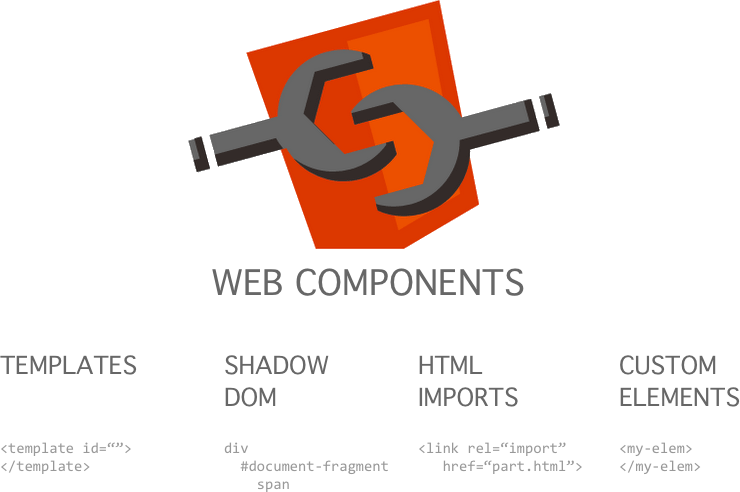
\includegraphics[width=1.0\linewidth]{images/chapter3/web_cmpts.png}\hfill
 \caption[Web Components]{Web Components}
 \label{fig:fourV}
\end{figure}
Web Components consist of 4 main elements which can be used separately or all together:
\begin{itemize}
\item Custom Elements: Custom Elements allow authors to define their own custom HTML elements. Authors associate JavaScript code with custom tag names, and then use those custom tag names as they would any standard tag.  Custom elements are still elements.  It is possible to create, use,
manipulate, and compose them just as easily as any standard <div> or <span> today.\cite{tch_custom}
\end{itemize}
\begin{itemize}
\item Shadow DOM: Shadow DOM addresses the lack of true DOM tree encapsulation when building components. With Shadow DOM, elements can get a new kind of node associated with them. This new kind of node is called a shadow root.  An element that has a “shadow root”  associated with it is called  a “shadow host”. The content of a shadow host isn’t rendered; the content of the shadow root is rendered instead.  Shadow DOM allows   a single node to express three subtrees:  light DOM, shadow DOM,  and composed DOM. Together, the light DOM and shadow DOM are referred to as the logical DOM. This is the DOM that the developer interacts with. The composed DOM is what the browser sees and uses to render the pixels on the  screen.\cite{tch_dom}
\newline
Structure of a Shadow DOM An element that has a shadow root asso- ciated with it is called shadow host. The shadow root can be treated as an ordinary DOM element, so it is possible to append arbitrary nodes to it. With Shadow DOM, all markup and CSS are scoped to the host element. In other words, CSS styles defined inside a Shadow Root won’t affect its parent document, CSS styles defined outside the Shadow Root won’t affect the main page.
\end{itemize}
\begin{itemize}
\item HTML Import: This webcomponents.js repository contains a  JavaScript  polyfill  for the HTML Imports specification. HTML Imports are a way to include and reuse HTML documents in other HTML documents. As <script> tags let authors include external JavaScript in their pages, imports let authors load full HTML resources. In particular, imports let authors include Custom Element definitions from external URLs.
\end{itemize}
\begin{itemize}
\item Templates: This specification describes a method for declaring inert DOM subtrees in HTML and manipulating them to instantiate document fragments with identical contents.
\end{itemize}